\documentclass[12pt]{book}
\usepackage[utf8]{inputenc}
\usepackage{amsmath, amssymb, amsthm}
\usepackage{graphicx}
\usepackage[normalem]{ulem}
\usepackage[a4paper,margin=1in]{geometry}
\usepackage{tikz, pgfplots}
\pgfplotsset{compat=1.18}

\theoremstyle{definition}
\newtheorem{exmp}{Example}[section]
\newtheorem{definition}{Definition}[section]
\newtheorem{theorem}{Theorem}[section]
\newtheorem{remark}{Remark}[section]
\newtheorem{corollary}{Corollary}[section]
\newtheorem{proposition}{Proposition}[section]

\title{Probability Theory Notes}
\author{Meow}

\setlength{\parindent}{1em}

\begin{document}

\maketitle
\chapter{Probability and Statistics}
\setcounter{section}{2}

\section{Basics of Statistics}
\begin{definition}
    A \textbf{class} is one of the categories into which quantitative data can be classified.
\end{definition}

Now, the \textbf{class frequency} is the number of observations in the data set falling in a particular class:
\begin{equation}
    \text{class relative frequency} = \frac{\text{class frequency}}{n}
\end{equation}

where \textit{n} is the total number of observations in the data set.

\begin{exmp}
    Consider the following data set of exam scores from a class of 20 students:
    \[ 65, 72, 68, 85, 90, 62, 75, 78, 80, 82, 88, 92, 95, 70, 73, 77, 81, 84, 89, 93 \]
    
    If we create classes with intervals of 10 points (60-69, 70-79, 80-89, 90-99), the class frequencies would be:
    \begin{itemize}
        \item 60-69: 3 scores (65, 68, 62)
        \item 70-79: 6 scores (72, 75, 78, 70, 73, 77)
        \item 80-89: 7 scores (85, 80, 82, 88, 81, 84, 89)
        \item 90-99: 4 scores (90, 92, 95, 93)
    \end{itemize}
    
    The relative frequencies would be:
    \begin{itemize}
        \item 60-69: 3/20 = 0.15 or 15\%
        \item 70-79: 6/20 = 0.30 or 30\%
        \item 80-89: 7/20 = 0.35 or 35\%
        \item 90-99: 4/20 = 0.20 or 20\%
    \end{itemize}
\end{exmp}

The mean of a sample of \( n \) measured responses \( y_1, y_2, \dots, y_n \) is:
\begin{equation}
    \bar{y} = \frac{1}{n} \sum_{i = 1}^{n} y_i
\end{equation}

The mean only shows the center of the distribution of the data. Different datasets may have equal means but different frequency distributions. In the figure below, what differs is the variation around the mean:
\begin{center}
    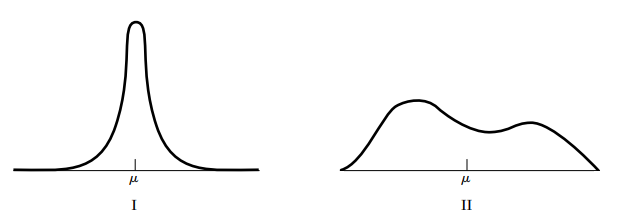
\includegraphics[scale=0.6]{../assets/distrib.png}
\end{center}

The \textbf{variance} of a sample \( y_1, y_2, \dots, y_n \) is the sum of squared differences between each measurement and the sample mean, divided by \( n - 1 \):
\begin{equation}
    s^2 = \frac{1}{n - 1} \sum_{i = 1}^{n} (y_i - \bar{y})^2
\end{equation}

It shows how much the data values vary compared to each other, in a dataset.

The \textbf{standard deviation} is the square root of the variance:
\begin{equation}
    s = \sqrt{s^2}
\end{equation}

It gives an accurate picture of how far apart the values in a dataset are from the mean.

For a distribution that is approximately bell-shaped, the following intervals apply:
\begin{itemize}
    \item \( \mu \pm \sigma \) contains approximately 68\% of the measurements.
    \item \( \mu \pm 2\sigma \) contains approximately 95\%.
    \item \( \mu \pm 3\sigma \) contains approximately all measurements.
\end{itemize}

\begin{center}
    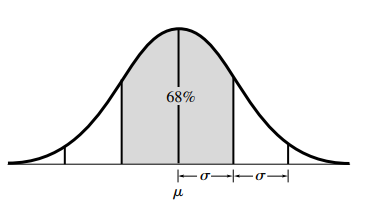
\includegraphics[scale=0.9]{../assets/bell-shape.png}
\end{center}

\begin{definition}
    The \textbf{range} of a sample of \textit{n} measurements $y_1, y_2, \dots, y_n$ is the difference between the largest and smallest measurements in the sample.
\end{definition}

\begin{exmp}
    If a sample consists of measurements 3, 1, 0, 4, 7, find the sample mean and range.

    \textbf{Solution}: 
    \[
        \text{Sample mean}: \frac{1}{5} \sum_{i = 1}^{5} y_i = 3
    \]
    \[
        \text{Range}: 7 - 0 = 7
    \]
\end{exmp}

\subsection{Normal Probability Distribution}
This distribution is symmetric to its mean $\mu$ and the spread is determined by the value of the standard deviation $\sigma$.
\begin{center}
    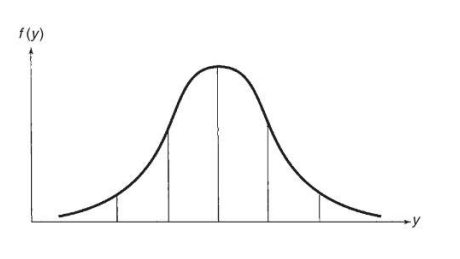
\includegraphics[scale=0.8]{../assets/normal-distrib.png}
\end{center}

The \textbf{z-score} measures the distance between the data points and the mean of the distribution, in number of standard deviations:
\begin{equation}
    z = \frac{y - \mu}{\sigma}
\end{equation}

But we can also use calculus to compute probabilities based on the z-score:
\begin{equation}
    P(a \leq X \leq b) = \int_{a}^{b} \frac{1}{\sqrt{2 \pi} \sigma} \, e^{-\frac{(x - \mu)^2}{2 \sigma^2}} \, dx
\end{equation}

\begin{exmp}
    Let $X \sim \mathcal{N}(100, 15^2)$. Find the probability that X lies between 85 and 115.

    \textbf{Solution}: \begin{equation}
        P(85 \leq X \leq 115) = \int_{85}^{115} \frac{1}{\sqrt{2 \pi} \cdot 15} \, e^{-\frac{(x - 100)^2}{2 \cdot 15^2}} \, dx
    \end{equation}
    which is equal to \textbf{0.6827} or 68.27\%.
\end{exmp}

\subsection{Sampling Distribution}
It's the distribution of all possible sample statistic computed from all possible samples of size \textit{n} from a population size of \textit{N}.

\begin{theorem}
    If $y_1, y_2, \dots, y_n$ represent a random sample of \textit{n} measurements from a large population with mean $\mu$ and standard deviation $\sigma$, the mean and standard error of estimate of the sampling distribution is:
    \begin{align*}
        \text{Mean }&: E(\bar{y}) = \mu \bar{y} = \mu \\
        \text{Standard error of estimate} &: \sigma \bar{y} = \frac{\sigma}{\sqrt{n}}
    \end{align*}
\end{theorem}

The \textbf{standard error} shows how different is the sample mean between different samples and the population itself.

\begin{theorem} [Central Limit Theorem]
    For large sample sizes, the mean $\bar{y}$ of a sample from a population with mean $\mu$ and standard deviation $\sigma$ has a sampling distribution approximately normal, regardless of the probability distribution of the sampled population. The larger the sample size, the better the approximation.
\end{theorem}


Now, the \textbf{covariance} demonstrates the direction of the linear relationship. It could be either positive or negative:

\begin{equation}
    \text{Covariance}(Y, X) = \frac{\sum_{i = 1}^{n} (y_i - \bar{y}) \cdot (x_i - \bar{x})}{(n-1)}
\end{equation}

Since covariance is affected by changes in the units of measurement, we standardize it:
\begin{equation}
    z_i = \frac{y_1 - \bar{y}}{s_y}
\end{equation}

where:
\begin{equation}
    s_y = \sqrt{\frac{\sum_{i = 1}^{n} (y_i - \bar{y})^2}{(n-1)}}
\end{equation}

is the \textbf{standard deviation} of \textit{Y}. We do the same for \textit{X}.

The \textbf{correlation coefficient} can be interpreted as the covariance of standardized variables:
\begin{equation}
    Cor(Y, X) = \frac{\sum (y_i - \bar{y} (x_i - \bar{x}))}{\sqrt{\sum (y_1 - \bar{y})^2 \sum (x_i - \bar{x})^2}}
\end{equation}

Correlation is useful to indicate both direction and strength of the linear relationship of your independent variables. The magnitude gives us the strength between Y and X. The closest the correlation is to -1 or 1, the strongest the relationship. The sign gives us the direction.
Having a correlation of 0 does not mean there's no relationship between the variables; it only means their relationship isn't \textbf{linear}.


\subsection{Confidence Interval}
When estimating a population parameter using a sample statistic, we'll always have some error because we're making approximations. To express that error, we use interval estimate:
\begin{equation}
    \text{Point estimate } \pm \text{Margin of error}
\end{equation}

A \textbf{confidence interval} is the range of values that likely contains the true population parameter. A \textbf{point estimate} is a single value used to estimate a population parameter. The \textbf{confidence level} is the percentage of all possible samples that can be expected to include the true population parameter. When the standard deviation is known the formula for the interval estimate is:

\begin{equation}
    \bar{y} \pm Z_{\frac{\alpha}{2}} \cdot \frac{\sigma}{\sqrt{n}}
\end{equation}

If the population standard deviation is unknown, we can use :

\begin{equation}
    \bar{y} \pm Z_{\frac{\alpha}{2}} \cdot \frac{s}{\sqrt{n}}
\end{equation}

\begin{center}
    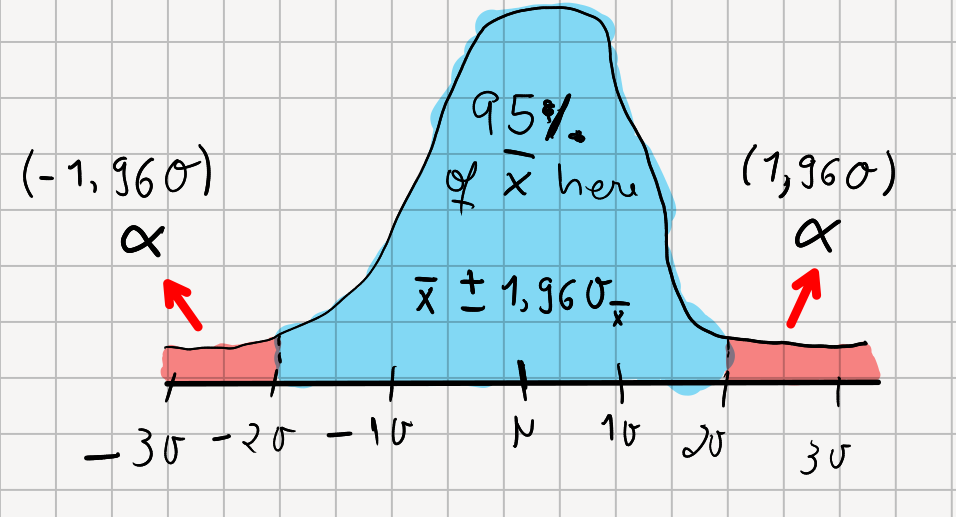
\includegraphics[scale=0.4]{../assets/confidence.png}
\end{center}

Since our $\alpha$ is in 2 parts of our distribution, we divide it by 2, getting 0.25\% on each side (our alpha is 5\% because we have a 95\% confidence interval in our case).

\begin{remark}
    We can only use the standard normal curve when we \textbf{know} the population standard deviation. Otherwise, we gotta use the t-distribution curve.
\end{remark}

Since the standard error depends on the sample size, our standard error of the mean will become larger and the distribution wider.

\begin{exmp}
    A coffee shop owner wants to estimate the average daily coffee consumption per customer. She randomly selected 50 customers and recorded their daily coffee consumption. The average is 2.3 cups and the sample standard deviation is 0.5 cups. She wants a 95\% confidence interval.

    \textbf{Solution}:

     \begin{equation}
       \bar{y} \pm Z_{\frac{\alpha}{2}} \cdot \frac{s}{\sqrt{n}} = 2.3 \pm 1.96 \cdot \frac{0.5}{\sqrt{50}} \approx 2.3 \pm 0.14
     \end{equation}

     The answer is 2.16 - 2.44 cups per customer, approximately, with 95\% confidence.
\end{exmp}

This large-sample method works when the sample size $\geq 30$, so that the sample standard deviation $\mu$ can be a good approximation of $\sigma$. When it's smaller, it's required that the sampled population have a normal probability distribution. We can use the \textbf{t-distribution}:
\begin{equation}
    \bar{y} \pm t_{\frac{\alpha}{2}} s_{\bar{y}}
\end{equation}

where $s_{\bar{y}} = \frac{s}{\sqrt{n}}$ is the estimated standard error of $\bar{y}$.

\subsection{Hypothesis Testing}
\label{subsec:hypothesis_testing}

Hypothesis testing is a statistical method used to evaluate claims about population parameters based on sample data.

\subsubsection*{Key Definitions}
\begin{itemize}
    \item \textbf{Null Hypothesis (H\textsubscript{0})}: The default assumption, postulated to be true unless evidence suggests otherwise. \\
    Example: \( H_0: \mu = \mu_0 \) (no effect or no difference).
    
    \item \textbf{Alternative Hypothesis (H\textsubscript{a})}: Counters the null hypothesis, representing the effect or difference we want to test. \\
    Examples:
    \begin{itemize}
        \item \( H_a: \mu > \mu_0 \) (one-tailed, right-tailed)
        \item \( H_a: \mu < \mu_0 \) (one-tailed, left-tailed)
        \item \( H_a: \mu \neq \mu_0 \) (two-tailed)
    \end{itemize}
\end{itemize}

\subsubsection*{Test Statistic}
A standardized value used to assess the null hypothesis:
\[
z = \frac{\bar{y} - \mu_0}{\sigma_{\bar{y}}}, \quad \text{where} \quad \sigma_{\bar{y}} = \frac{\sigma}{\sqrt{n}}
\]
\begin{itemize}
    \item \(\bar{y}\): Sample mean
    \item \(\mu_0\): Hypothesized population mean under \( H_0 \)
    \item \(\sigma_{\bar{y}}\): Standard error of the mean (measures sampling variability)
\end{itemize}

\subsubsection*{Decision Rules}
\begin{enumerate}
    \item \textbf{Rejection Region Approach:} \\
    Compare the test statistic (\( z \)) to a critical value (\( z_{\alpha} \)) based on the chosen significance level (\( \alpha \)).
    \begin{itemize}
        \item For \( H_a: \mu > \mu_0 \), reject \( H_0 \) if \( z > z_{\alpha} \).
        \item For \( H_a: \mu < \mu_0 \), reject \( H_0 \) if \( z < -z_{\alpha} \).
        \item For \( H_a: \mu \neq \mu_0 \), reject \( H_0 \) if \( |z| > z_{\alpha/2} \).
    \end{itemize}
    
    \item \textbf{p-Value Approach:} \\
    \textbf{p-value}: Probability of observing a test statistic as extreme as (or more extreme than) the sample result, assuming \( H_0 \) is true. \\
    \textbf{Rule}: Reject \( H_0 \) if \( p\text{-value} < \alpha \).
\end{enumerate}

\subsubsection*{Errors in Hypothesis Testing}
\begin{itemize}
    \item \textbf{Type I Error (\(\alpha\))}: Rejecting \( H_0 \) when it is true (false positive).
    \item \textbf{Type II Error (\(\beta\))}: Failing to reject \( H_0 \) when it is false (false negative).
    \item \textbf{Power (\(1-\beta\))}: Probability of correctly rejecting \( H_0 \) when \( H_a \) is true.
\end{itemize}

\subsection{Confidence Interval for Two Populations}
To construct a confidence interval for two populations, we use the difference of their means.
For large samples ($n \geq 30$), the sampling distribution of the sample means $\bar{x}_1 \text{ and } \bar{x}_2$ is approximately normal and we use the \textit{z-score} as our test statistic. The variance of the populations are rarely known so we use their variances to estimate the population mean:

\begin{equation}
    (\bar{x}_1 - \bar{x}_2) \pm z_{\frac {\alpha} {2}} \sigma_{\bar{x}_1 - \bar{x}_2} = (\bar{x}_1 - \bar{x}_2) \pm z_{\frac {\alpha} {2}} \sqrt{\frac{\sigma_1^2} {n_1} + \frac{\sigma_2^2} {n_2}}
\end{equation}

We're assuming here that the samples were randomly and independently selected and their sizes are large enough so that their sampling distributions are approximately normal.

\begin{exmp}
    A technology company is evaluating the feasibility of expanding its operations in either São Paulo or Rio de Janeiro. To compare the average annual salaries of software engineers in these two cities, the company collects two independent random samples:

    \begin{itemize}
    \item \textbf{São Paulo (Population 1):}
    \begin{itemize}
        \item Sample size: $n_1 = 100$
        \item Sample mean salary: $\bar{x}_1 = \text{R\$}120{,}000$
        \item Sample standard deviation: $s_1 = \text{R\$}15{,}000$
    \end{itemize}

    \item \textbf{Rio de Janeiro (Population 2):}
    \begin{itemize}
        \item Sample size: $n_2 = 120$
        \item Sample mean salary: $\bar{x}_2 = \text{R\$}112{,}000$
        \item Sample standard deviation: $s_2 = \text{R\$}18{,}000$
    \end{itemize}
    \end{itemize}

    Assume both samples are independent, random, and sufficiently large such that the Central Limit Theorem applies.

    \bigskip

    \textbf{Question:} Construct a 95\% confidence interval for the difference in mean salaries, $\mu_1 - \mu_2$, between São Paulo and Rio de Janeiro.
\end{exmp}

\subsection{Chi-square Test}
The chi-square ($\chi^2$) test determines whether there is a statistically significant association between two categorical variables by comparing observed frequencies to expected frequencies under the null hypothesis.

A school principal would like to know in which days of the week the students are more likely to be absent. The principal expects that students will be absent equally during the 5-day school week. The principal selects a random sample of 100 teachers asking them which day of the week they had the highest number of student absences. The observed and expected results are shown below. Based on these days, do the days for the highest number of absences occur with equal frequencies? (Use a 5\% significance level).

\begin{table}[h]
    \centering
    \caption{Observed vs. Expected Student Absences by Weekday}
    \begin{tabular}{|l|c|c|}
    \hline
    \textbf{Day of Week} & \textbf{Observed Absences} & \textbf{Expected Absences} \\ \hline
    Monday    & 25 & 20 \\ \hline
    Tuesday   & 15 & 20 \\ \hline
    Wednesday & 20 & 20 \\ \hline
    Thursday  & 18 & 20 \\ \hline
    Friday    & 22 & 20 \\ \hline
    \textbf{Total} & \textbf{100} & \textbf{100} \\ \hline
    \end{tabular}
    \label{tab:absences}
    
    \smallskip
    $H_0$: Equal frequencies of absences across weekdays \\
    $H_a$: Unequal frequencies of absences across weekdays
\end{table}

The Chi-squared distribution is an uneven distribution.

\begin{center}
    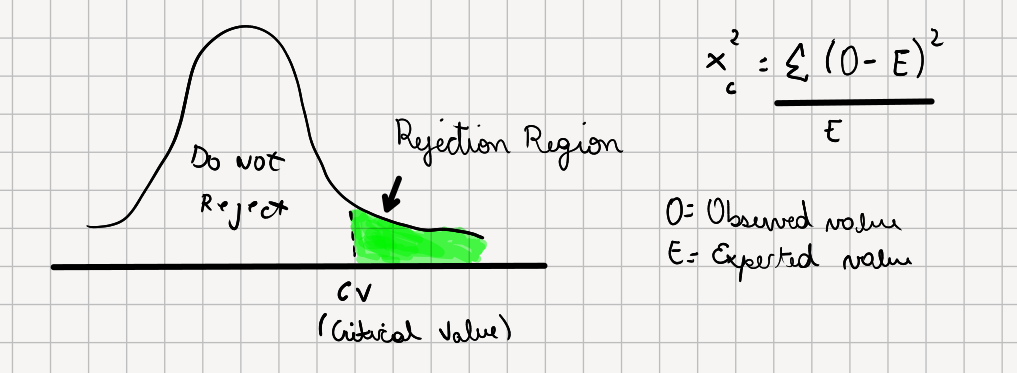
\includegraphics[scale=0.4]{../assets/chi-squared.png}
\end{center}


\subsection{Simple Linear Regression Model}
The linear regression model expresses the relationship between \textit{Y} and \textit{X} as shown below:
\begin{equation}
    Y = B_0 + B_1X_i + \epsilon
\end{equation}

where $B_0$ is the y-intercept, $B_1$ is the slope and $\epsilon$ accounts for the error in the approximation (the random disturbance). The word \textbf{linear} could mean that the relationship between \textit{Y} and \textit{X} is linear, but it could also mean that the coefficients enter in a linear fashion in the model.

To estimate the parameters, we find the best fitting line of the points in our scatter plot. For that, we can use the \textit{least squares method}, which gives us the line that minimizes the sum of squares of the difference between the observed values and the estimations:
\begin{equation}
    \epsilon_i = y_i - \beta_0 - \beta_1X_i
\end{equation}

The sum is:
\begin{equation}
    S(B_0, B_1) = \sum \epsilon_i^2 = \sum (y_i - \beta_0 - \beta_1 X_i)^2
\end{equation}

To minimize it we can use:
\begin{equation}
    B_1 = \frac{\sum (y_i - \bar{y})(x_i - \bar{x})}{\sum (x_i - \bar{x})^2}
\end{equation}

and:
\begin{equation}
    \beta_0 = \bar{y} - \hat{\beta}_1\bar{x}
\end{equation}

\section{Basics of set theory}
Let $\Omega$ denote the sample space, and let $\omega$ denote an element of that sample space. We say that $\omega$ is an element of $\Omega$, written as $\omega \in \Omega$. The negation, indicating that $\omega$ is not an element of $\Omega$, is written as $\omega \notin \Omega$.

A set $A$ is a \textit{subset} of $\Omega$ if every element of $A$ is also an element of $\Omega$; that is,
\[
A \subseteq \Omega \iff \forall \omega \in A,\; \omega \in \Omega.
\]

A set $A$ is a \textit{proper subset} of $\Omega$, denoted by $A \subset \Omega$, if it is a subset of $\Omega$ but not equal to $\Omega$. Formally,
\[
A \subset \Omega \iff A \subseteq \Omega \land A \neq \Omega.
\]

The \textit{complement} of \textit{A}, denoted by $\textit{A}^c$ represents all elements that do not belong in A. The \textit{union} represents all elements that are in at least one of the sets: 
\[
    A_1 \cup A_2 \dots \cup A_n = \bigcup_{i = 1}^{n} A_i \quad \text{ with } i = 1, 2, \dots, n
\]

The \textbf{intersection} of two sets $A_1$ and $A_2$, denoted by:
\[
    A_1 \cap A_2
\] represents the elements belonging to both sets. We can further extend this notion for any number of sets:
\[
    A_1 \cap A_2 \cap \dots \cap A_n = \bigcap_{i = 1}^{n}, \text{ with } i = 1, 2, \dots, n
\]

\begin{theorem}
    For any three events A, B and C, defined on a sample space $\Omega$:

    \begin{enumerate}
        \item Commutativity
        \begin{itemize}
            \item $A \cup B = B \cup A$
            \item $A \cap B = B \cap A$
        \end{itemize}

        \item Associativity
        \begin{itemize}
            \item $A \cup (B \cup C) = (A \cup B) \cup C$
            \item $A \cap (B \cap C) = (A \cap B) \cap C$
        \end{itemize}

        \item Distributive
        \begin{itemize}
            \item $A \cup (B \cap C) = (A \cap B) \cup (A \cap C)$
            \item $A \cap (B \cup C) = (A \cup B) \cap (A \cup C)$
        \end{itemize}

        \item DeMorgan's Laws
        \begin{itemize}
            \item $(A \cup B)^c = A^c \cap B^c$
            \item $(A \cap B)^c = A^c \cup B^c$
        \end{itemize}
    \end{enumerate}
\end{theorem} 

To prove the distributive law \( A \cap (B \cup C) = (A \cap B) \cup (A \cap C) \), we establish set equality by proving containment in both directions. First, suppose \( x \in A \cap (B \cup C) \). Then \( x \in A \) and \( x \in B \cup C \), meaning \( x \in B \) or \( x \in C \). If \( x \in B \), then \( x \in A \cap B \); if \( x \in C \), then \( x \in A \cap C \). In either case, \( x \in (A \cap B) \cup (A \cap C) \), proving \( A \cap (B \cup C) \subseteq (A \cap B) \cup (A \cap C) \).

Conversely, let \( x \in (A \cap B) \cup (A \cap C) \). Then \( x \in A \cap B \) or \( x \in A \cap C \). If \( x \in A \cap B \), then \( x \in A \) and \( x \in B \), so \( x \in B \cup C \), implying \( x \in A \cap (B \cup C) \). Similarly, if \( x \in A \cap C \), then \( x \in A \) and \( x \in C \), so \( x \in B \cup C \), again implying \( x \in A \cap (B \cup C) \). Thus, \( (A \cap B) \cup (A \cap C) \subseteq A \cap (B \cup C) \). Since both inclusions hold, the equality follows.

\begin{definition}
    Two events $A$ and $B$ are \textit{disjoint} if their intersection is empty. Also, two events $A_1, A_2, \dots$ are \textit{pairwise disjoint} if $A_i \cap A_j = \emptyset, \forall i \neq j$.
\end{definition}

\begin{definition}
    If $A_1, A_2, \dots$ are pairwise disjoint and $\bigcup_{i = 1}^{\infty} A_i = \Omega$, then the collection $A_1, A_2, \dots$ forms a \textbf{partition} of the sample space.
\end{definition}

\subsection{Sequences and Their Limits}
Monotone sequences can be classified as either \textbf{nondecreasing} or \textbf{nonincreasing}.

\subsubsection{Nondecreasing Sequences}
A sequence of sets $\{A_n\}$ is \textbf{nondecreasing} if:
\[
A_n \subseteq A_{n+1} \quad \text{for all } n \in \mathbb{N}
\]
The limit of such a sequence is given by:
\[
\lim_{n \to \infty} A_n = \bigcup_{n=1}^{\infty} A_n
\]

For a numerical sequence $\{a_n\}$, nondecreasing means:
\[
a_{n+1} \geq a_n \quad \forall n \in \mathbb{N}
\]
\textbf{Example:}
\[
a_n = n \quad \text{yields} \quad 1, 2, 3, 4, \dots
\]

\subsubsection{Nonincreasing Sequences}
A sequence of sets $\{A_n\}$ is \textbf{nonincreasing} if:
\[
A_n \supseteq A_{n+1} \quad \text{for all } n \in \mathbb{N}
\]
The limit in this case is:
\[
\lim_{n \to \infty} A_n = \bigcap_{n=1}^{\infty} A_n
\]

\textbf{Numerical Example:}
\[
b_n = \frac{1}{n} \quad \text{yields} \quad 1, \frac{1}{2}, \frac{1}{3}, \frac{1}{4}, \dots
\]

\begin{center}
\boxed{
\begin{aligned}
&\text{\textbf{Key Properties:}} \\
&\bullet \text{ Nondecreasing: } \limsup A_n = \liminf A_n = \bigcup_{n=1}^\infty A_n \\
&\bullet \text{ Nonincreasing: } \limsup A_n = \liminf A_n = \bigcap_{n=1}^\infty A_n
\end{aligned}
}
\end{center}


\subsection{Probability of Unions, complements and intersections}
\[
    P(A \cup B) = P(A) + P(B) - P(A \cap B)
\]

If \textit{A} and \textit{B} are mutually exclusive:
\[
    P(A \cup B) = P(A) + P(B)
\]

for complements:
\[
    P(A^c) = 1 - P(A)
\]

Two events are \textbf{independent} if and only if the probability of occurrence of event B has no effect on the probability of occurrence of A, and vice-versa.

\subsection{Probability Measure}
A \textbf{probability measure} or \textbf{probability distribution} is a function that assigns for each event \textit{A} a real number and satisfies three axioms:

\begin{enumerate}
    \item $\mathcal{P}(A) \geq 0$
    \item $\mathcal{P}(\Omega) = 1$
    \item If $A_1, A_2, \dots$ are disjoint, then: 
    \[
        \mathcal{P}(\bigcup_{i = 1}^{\infty} A_i) = \sum_{i = 1}^{\infty} \mathcal{P}(A_i)
    \]
\end{enumerate}

\subsection{Conditional Probability}
We can reason about the outcome of an experiment, based on partial information:
\begin{exmp}
    In a word guessing game, the first letter of the word is \textit{h}. What's the probability that the second letter is an \textit{h}?
\end{exmp}

The formula is:
\begin{equation}
    P(A|B) = \frac{\text{number of elements of $A \cap B$}}{\text{number of elements of B}}
\end{equation}

which corrresponds to:
\begin{equation}
    P(A|B) = \frac{P(A \cap B)}{P(B)}
\end{equation}

where we assume that $P(B) \geq 0$.

\begin{exmp}
    We toss a fair coin three successive times. We want to find the conditional probability $P(A|B)$, where A and B are the events:
    \[
        A = \{\text{more heads than tails come up}\}, \quad B = \{\text{1st toss is a head}\}
    \]

    The sample space is:
    \[
        \Omega = \{HHH, HHT, HTH, HTT, THH, THT, TTH, TTT\}
    \]

    Event \textit{B} consists of 4 events: 
    \[
        \{HHH, HHT, HTH, HTT\}
    \]

    If we assume they're equally likely:
    \[
        P(B) = \frac{4}{8}
    \]

    Now, $P(A \cap B)$ consists of three elements:
    \[
        P(A \cap B) = \{HHH, HHT, HTH\} = \frac{3}{8}
    \]

    So, the conditional probability of \textit{A} given \textit{B} is:
    \[
        P(A|B) = \frac{\frac{3}{8}}{\frac{4}{8}} = \frac{3}{4}
    \]
\end{exmp}

We can extend this notion to \textit{n} events:
\begin{equation}
    P(\bigcap_{i = 1}^{n} A_i) = P(A_1) \cdot \frac{P(A_1 \cap A_2)}{P(A_1)} \cdot \frac{P(A_1 \cap A_2 \cap A_3)}{P(A_1 \cap A_2)} \cdot \dots \frac{P(\bigcap_{i = 1}^{n} A_1)}{P(\bigcap_{i = 1}^{n-1}A_i)}
\end{equation}

Events \textit{A} and \textit{B} are \textbf{conditionally independent} given event \textit{C} if:
\[
    P(A,B | C) = P(A|C)P(B|C)
\]

\subsection{Random Variables}
If $X$ represents some unknown value of interest or if this value could change, we have a \textbf{random variable}. The set $\mathcal{X}$ represents all the possible values for \textit{X}. When the sample space $\mathcal{X}$ is finite or countably infinite, \textit{X} is a \textbf{discrete random variable}. Then, the probability of \textit{X} having value \textit{x} is denoted by:
\[
    P(X = x)
\]

\subsubsection{Probability mass function} 
It describes the probabilities of possible discrete outcomes for our random variable. Some conditions must be met:
\begin{itemize}
    \item $0 \leq P(X = x) \leq 1$
    \item $\sum_{\text{all } x} P(X = x) = 1$
\end{itemize}

If $X \in \mathbb{R}$ we use \textbf{probability density function} instead.

\subsubsection{Cumulative probability distributions}
They're used to calculate the area under the curve to the left of a point of interest. It's used to evaluate the accumulated probability.

\[
    F_X(x) = P(X \leq x) = \int_{- \infty}^{x} f_X(t) dt
\]

Let us consider a rectangular distribution, also called a \textbf{uniform distribution}.

\begin{center}
    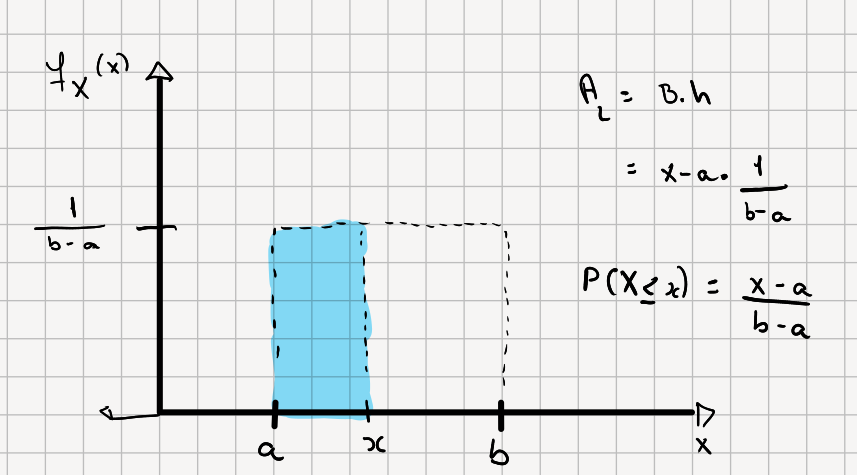
\includegraphics[scale=0.5]{../assets/cdf.png}
\end{center}

% Talk about exponential distributions and how to find the pdf and cdf

\subsection{Expectation}
The \textbf{expected value} is the mean of the random variable:

\[
    E(X) = \mu = \sum xP(x)
\]

\end{document}
